
\subsection{Cyclic Extensions}
In this subsection we prove the following. 
\begin{thm}\label{thm_consistent_cyclic}
    Let $E/\QQ$ be a semistable elliptic curve and let $F$ be a finite cyclic Galois extension $\QQ$ so that $\Gal(F/\QQ)=C_d$ for some $d\geq 2$. Let $\chi$ be a faithful character of $C_d$ (so that $\QQ(\chi)=\QQ(\zeta_d)$), and let $F_i,F'_j\subseteq F$ be such that
    $$\bigoplus_{\mathfrak{g}\in\Gal(\QQ(\zeta_d)/\QQ)}\chi^{\mathfrak{g}}=\bigoplus_i\Ind_{F_i/\QQ}\mathds{1}\ominus\bigoplus_j\Ind_{F'_j/\QQ}\mathds{1}.$$
    Then for any $\QQ(\sqrt{D})\subseteq\QQ(\zeta_d)$,
    $$\frac{\prod_i C_{E/F_i}}{\prod_j C_{E/F_j'}}$$
    is a norm of $\QQ(\sqrt{D})$. Moreover, the contribution is always the square of rational number unless $d=2^n, p^n,2p^n$ for some odd prime $p$.
\end{thm}

The first step in proving Theorem \ref*{thm_consistent_cyclic} is to show that the fields $F_i, F'_j$ exist, and to give a precise description. Recall that for each $k\mid d$ the cyclic group $C_d$ has one unique subgroup of order $k$, which is of course also cyclic. Therefore, for each $k\mid d$, there is one unique subfield $L_k$ of $F$ of degree $k$ over $\QQ$ which is also cyclic. Under the Galois correspondence, this field corresponds to the subgroup $H_k=\Gal(F/L_k)=C_{d/k}$.

To give the required description, we recall that the Möbius function $\mu$ is the function supported on the square-free integers, and $\mu(n)=(-1)^s$ whenever $n$ is square free and $s$ is the number of prime factors of $n$.

\begin{lemma}\label{lem_cyclic_decomp}
    Let $E/\QQ$, $F$ and $\chi$ be as in Theorem \ref*{thm_consistent_cyclic}. Writing characters of $C_d$ additively, we have that
    \begin{equation}\label{eqn_cyclic_relation}
        \sum_{\mathfrak{g}\in\Gal(\QQ(\zeta_d)/\QQ)}\chi^{\mathfrak{g}}=\sum_{k\mid d}\mu(d/k)\Ind_{L_k/\QQ}\mathds{1}.
    \end{equation}
    Furthermore, such an expression is unique.
\end{lemma}

\begin{rem}\label{rem_radical}
    This lemma has an important consequence. Given an integer $d\geq2$, let $\rad(d)=\prod_{p\mid d}p$ be the radical of $d$, and let $K=L_{d/\rad(d)}$ be the unique subfield of $F$ such that $[F:K]=\rad(d)$. For $k\mid d$, $\mu(d/k)\neq 0$ precisely when $[K:\QQ]=\frac{d}{\rad(d)}\mid k$ and therefore the fields appearing in the right hand side of \eqref{eqn_cyclic_relation} are the fields $L_k$ satisfying $K\subseteq L_k\subseteq F$. 
\end{rem}

Following this observation, we will compute the product of the local factors locally for each finite place $\pp$ of $K$ and the places above it in the other fields $L_k\supseteq K$. To that objective, the following notation will be useful.

\begin{notation}\label{not_local_contr}
    Let $E/\QQ$, $F$ and $\chi$ be as in Theorem \ref*{thm_consistent_cyclic}, and let $L_k$ and $K$ be as in Remark \ref*{rem_radical}. For a finite place $\pp$ of $K$, we write
    $$\contr_\chi(\pp)=\prod_{\frac{d}{\rad(d)}\mid k\mid d}C_{\mathfrak{P}\mid\pp}(L_k/K)^{\mu(d/k)}=\prod_{k\mid d}C_{\mathfrak{P}\mid\pp}(L_k/K)^{\mu(d/k)}$$ 
    where the terms in the product are defined as in Notation \ref*{not_contr}. 
\end{notation}

An immediate consequence of the above definition is the fact that 
\begin{equation}\label{eqn_local_contr}
    \prod_{k\mid d}(C_{E/L_k})^{\mu(d/k)}=\prod_\pp\contr_\chi(\pp),
\end{equation}

and therefore we can calculate the product of local terms \textbf{locally}, one prime $\pp$ at a time.

We divide the proof of Theorem \ref*{thm_consistent_cyclic} into two cases: odd and even cyclic extensions. The main idea in both cases is to simplify the general case into smaller cases where we can directly compute $\contr_\chi(\pp)$ for each finite place $\pp$ of $K$. We note that if $E$ has good reduction over $\pp$, then $\contr_\chi(\pp)=1$ and therefore we focus our attention to bad semistable reduction. 

\subsection*{Odd Cyclic Extensions} \label{case_Cp}

For the first case, we assume that $d$ is odd. Following the observation in Remark \ref*{rem_radical}, we need to calculate $\contr_\chi(\pp)$ for each finite place $\pp$ of $K$. To that objective, we first calculate them for ``small'' cases and then we use them for the general case. The following lemmas build on this idea.

\begin{lemma}\label{lem_Cp}
    Let $p$ be a rational prime, $F/K$ a Galois extension of number fields such that $\Gal(F/K)=C_p$ and $E/\QQ$ an elliptic curve with semistable reduction at $2$ and $3$. Then 
    $$\frac{C_{E/F}}{C_{E/K}}$$
    is a rational square up factors of $p$.
\end{lemma}

\begin{proof}
    Fix some prime $\pp$ in $K$. Since the extension $L/K$ is cyclic, the splitting behaviour in $L$ is determined by the ramification index $e_\pp$ and the residual degree $f_\pp$. Since $\contr_\chi(\pp)=1$ if $E$ has good reduction at $\pp$ and $E$ is assumed to be semistable, we assume that $E$ has split or non-split multiplicative reduction. The following table records the contribution of $\pp$ dependinng on $e_\pp$ and $f_\pp$, and the entries for split and non-split multiplicative reduction of type $\mathrm{I}_n$ are separated by a ``;''.
    \begin{table}[h!]
        \centering
        \begin{tabular}{|l|l|l|l|l|}
        \hline
        $e_\pp$ & $f_\pp$  & $C_{\mathfrak{P}\mid \pp}(K/K)$ & $C_{\mathfrak{P}\mid \pp}(F/K)$  & $\contr_\chi(\pp)$ \\ \hline
        $1$ & $1$ & $n;\tilde{n}$ & $n^p;\tilde{n}^p$ & $\square$ \\ \hline
        $p$ & $1$ & $n;\tilde{n}$ & $pn;\tilde{n}$ & $p\square;\square$ \\ \hline
        $1$ & $p$ & $n;\tilde{n}$ & $n;\tilde{n}$ & $\square$ \\ \hline
        \end{tabular}
    \end{table}
    The proof follows immediately from \eqref{eqn_local_contr}.
\end{proof}

Next, we prove an analogous result for $C_{pq}$ extensions, where $p$ and $q$ are odd rational primes.

\begin{lemma}\label{lem_Cpq}
    Let $p,q$ be distinct, odd rational primes and let $F/K$ be a Galois extension of number fields such that $\Gal(F/K)=C_{pq}$. Let $E/\QQ$ be an elliptic curve with semistable reduction at $2$ and $3$ and let $L_k$ be the fields as above. Then
    $$\frac{C_{E/F}C_{E/K}}{C_{E/L_p}C_{E/L_q}}$$
    is always a rational square.
\end{lemma}

\begin{proof}
    The idea of the proof is identical to Lemma \ref*{lem_Cp} since in a $C_{pq}$ extension $L/K$ the splitting behaviour of a prime $\pp$ of $K$ in $L$ and all the intermediate fields is determined by $e_\pp$ and $f_\pp$. The following table records the contribution of $\pp$ depending on these values, and again the entries for split and non-split multiplicative reduction of type $\mathrm{I}_n$ are separated by ``;''.

    \begin{table}[!ht]
        \centering
        \begin{tabular}{|l|l|l|l|l|l|l|}
        \hline
        $e_\pp$ & $f_\pp$  & $C_{\mathfrak{P}\mid \pp}(K)$ & $C_{\mathfrak{P}\mid \pp}(L_p)$ & $C_{\mathfrak{P}\mid \pp}(L_q)$ & $C_{\mathfrak{P}\mid \pp}(F)$ & $\contr_\chi(\pp)$ \\ \hline
        $1$ & $1$ & $n;\tilde{n}$ & $n^p;\tilde{n}^p$ & $n^q;\tilde{n}^q$ & $n^{pq};\tilde{n}^{pq}$ & $\square$ \\ \hline
        $1$ & $p$ & $n;\tilde{n}$ & $n;\tilde{n}$ & $n^q;\tilde{n}^q$ & $n^q;\tilde{n}^q$ & $\square$ \\ \hline
        $1$ & $q$ & $n;\tilde{n}$ & $n^p;\tilde{n}^p$ & $n;\tilde{n}$ & $n^p;\tilde{n}^p$ & $\square$ \\ \hline
        $1$ & $pq$ & $n;\tilde{n}$ & $n;\tilde{n}$ & $n;\tilde{n}$ & $n;\tilde{n}$ & $\square$ \\ \hline
        $p$ & $1$ & $n;\tilde{n}$ & $pn;\tilde{n}$ & $n^q;\tilde{n}^q$ & $p^qn^q;\tilde{n}^q$ & $\square$ \\ \hline
        $p$ & $q$ & $n;\tilde{n}$ & $pn;\tilde{n}$ & $n;\tilde{n}$ & $pn;\tilde{n}$ & $\square$ \\ \hline
        $q$ & $1$ & $n;\tilde{n}$ & $n^p;\tilde{n}^p$ & $qn;\tilde{n}$ & $q^pn^p;\tilde{n}^p$ & $\square$ \\ \hline
        $q$ & $p$ & $n;\tilde{n}$ & $n;\tilde{n}$ & $qn;\tilde{n}$ & $qn;\tilde{n}$ & $\square$ \\ \hline
        $pq$ & $1$ & $n;\tilde{n}$ & $pn;\tilde{n}$ & $qn;\tilde{n}$ & $pqn;\tilde{n}$ & $\square$ \\ \hline
        \end{tabular}
    \end{table}
Again, the result follows immediately from the table and \eqref{eqn_local_contr}.
    \begin{figure}[!ht]
        \centering
        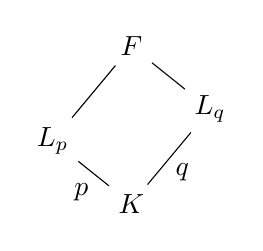
\begin{tikzpicture}

            \node (Q1) at (0,0) {$K$};
            \node (Q2) at (1,1.2) {$L_q$};
            \node (Q3) at (0,2) {$F$};
            \node (Q4) at (-1,0.8) {$L_p$};
        
            \draw (Q1)--(Q2) node [pos=0.8, below,inner sep=0.25cm] {$q$};
            \draw (Q1)--(Q4) node [pos=0.9, below,inner sep=0.25cm] {$p$};
            \draw (Q3)--(Q4);
            \draw (Q2)--(Q3);
        
        \end{tikzpicture}
        \caption[short]{Subfields of a $C_{pq}$-extension}
    \end{figure}
\end{proof}

We are finally ready to prove the main result of this section, from which Theorem \ref*{thm_consistent_cyclic} will follow. 

\begin{lemma}\label{lem_Cd_odd}
    Let $d$ be a composite, odd squarefree integer and let $F/K$ be a Galois extension of number fields such that $\Gal(F/K)=C_{d}$. Let $E/\QQ$ be an elliptic curve and let $L_k$ be the fields as above. Then
    $$\prod_{k\mid d}(C_{E/L_k})^{\mu(d/k)}$$
    is always a rational square.
\end{lemma}

\begin{proof}
    Let $n$ be the number of distinct prime numbers dividing $d$, so that $d=p_1\ldots p_n$ for some distinct odd primes $p_i$. We prove this result by induction. The base case for $n=2$ is the content of Lemma \ref*{lem_Cpq}. Assume that the result holds for squarefree integers with $n-1$ prime factors and consider the two sets of fields
    $$\mathcal{A}=\{L_k:p_n\nmid k\}\quad\text{and}\quad\mathcal{B}=\{L_k:p_n\mid k\},$$
    which are clearly a partition of all intermediate fields of $F/K$. Furthermore, the fields in $\mathcal{A}$ are precisely the intermediate fields of $K$ and $L_{d/p_n}$, while the fields in $\mathcal{B}$ are the intermediate fields of $L_{p_n}$ and $F$. However, since $\Gal(L_{d/p_n}/K)=\Gal(F/L_{p_n})=C_{d/p_n}$, it follows from the inductive hypothesis applied to the fields of $\mathcal{A}$ and $\mathcal{B}$ respectively that
    $$\prod_{k\mid \frac{d}{p_n}}(C_{E/L_k})^{\mu\left(\frac{d}{kp_n}\right)}\quad\text{and}\quad\prod_{p_n\mid k\mid d}(C_{E/L_{k}})^{\mu\left(d/k\right)}$$
    are both rational squares. By the natural decomposition
    $$\prod_{k\mid d}(C_{E/L_k})^{\mu(d/K)}=\prod_{k\mid \frac{d}{p_n}}(C_{E/L_k})^{\mu\left(d/k\right)}\prod_{p_n\mid k\mid d}(C_{E/L_{k}})^{\mu\left(d/k\right)}=\left(\prod_{k\mid \frac{d}{p_n}}(C_{E/L_k})^{\mu\left(\frac{d}{kp_n}\right)}\right)^{-1}\prod_{p_n\mid k\mid d}(C_{E/L_{k}})^{\mu\left(d/k\right)},$$
    it follows that the left hand side is also a rational square, as desired.
    \begin{figure}[!ht]
        \centering
        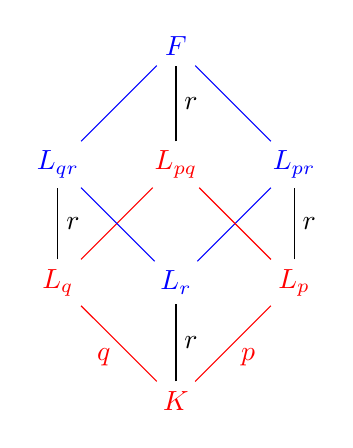
\begin{tikzpicture}

            \node [red] (Q1) at (0,0) {$K$};
            \node [red] (Q2) at (-1.5,1.5) {$L_q$};
            \node [blue] (Q3) at (0,1.5) {$L_r$};
            \node [red] (Q4) at (1.5,1.5) {$L_p$};
            \node [blue] (Q5) at (-1.5,3) {$L_{qr}$};
            \node [red] (Q6) at (0,3) {$L_{pq}$};
            \node [blue] (Q7) at (1.5,3) {$L_{pr}$};
            \node [blue] (Q8) at (0,4.5) {$F$};

            \draw [red] (Q1)--(Q2) node [pos=0.7, below,inner sep=0.25cm] {$q$};
            \draw [red] (Q1)--(Q4) node [pos=0.7, below,inner sep=0.25cm] {$p$};
            \draw (Q1)--(Q3) node [pos=0.5, right,inner sep=0.1cm] {$r$};
            \draw (Q2)--(Q5) node [pos=0.5, right,inner sep=0.1cm] {$r$};
            \draw (Q2)--(Q6) [red];
            \draw (Q3)--(Q5) [blue];
            \draw (Q3)--(Q7) [blue];
            \draw (Q4)--(Q6) [red];
            \draw (Q4)--(Q7) node [pos=0.5, right,inner sep=0.1cm] {$r$};
            \draw (Q5)--(Q8) [blue];
            \draw (Q6)--(Q8) node [pos=0.5, right,inner sep=0.1cm] {$r$};
            \draw (Q7)--(Q8) [blue];
        
        \end{tikzpicture}
        \caption[short]{Partition of $n=3$ into $n=2$. Red fields are in $\mathcal{A}$ while blue fields are in $\mathcal{B}$.}
    \end{figure}
\end{proof}

We are now ready to prove Theorem \ref*{thm_consistent_cyclic} for odd $d$.

\begin{proof}[Theorem \ref*{thm_consistent_cyclic} for odd $d$]
    The proof is divided into two cases depending on whether $d$ is the power of a prime or not. Suppose first that $d$ is not, so that $\rad(d)$ is a squarefree \textbf{composite} number. However, by Remark \ref*{rem_radical} and Lemma \ref*{lem_Cd_odd} we know that 
    $$\frac{\prod_i C_{E/F_i}}{\prod_j C_{E/F'_j}}$$
    is a rational square, and therefore it is the norm of an element for any quadratic extension of $\QQ$. 

    The case when $d=p^n$ for some odd prime $p$ and $n\geq1$ requires some more work. Lemma \ref*{lem_cyclic_decomp} and Lemma \ref*{lem_Cp} show that 
    $$\frac{\prod_i C_{E/F_i}}{\prod_j C_{E/F'_j}}=\frac{C_{E/F}}{C_{E/L_{p^{n-1}}}}$$
    is a rational square up to factors of $p$. Therefore, it suffices to show that $p$ is the norm of any quadratic subextension of $\QQ(\zeta_{p^n})$. Since $\Gal(\QQ(\zeta_{p^n})/\QQ)=(\ZZ/p^n\ZZ)$ is cyclic, $\QQ(\zeta_{p^n})$ has one unique quadratic subextension. Hence, it suffices to find the unique quadratic subextension of $\QQ(\zeta_p)$. A simple calculation shows that 
    $$\left(\sum_{a=0}^{p-1}\left(\frac{a}{p}\right)\zeta_p^a\right)^2=(-1)^{(p-1)/2}p,$$
    and therefore $\QQ(\sqrt{p^*})$ is the unique quadratic subextension of $\QQ(\zeta_p)$, where $p^*=(-1)^{(p-1)/2}p$. The fact that $p$ is a norm in this field is precisely the content of Corollary \ref*{p-norm}, and so the Theorem follows.
\end{proof}
 
\subsection*{Even Cyclic Extensions}
A bit more care is required to prove Theorem \ref*{thm_consistent_cyclic} for even $d$. This difficulty mainly lies in the case when $d$ is only divisible by one odd prime $p$. Likewise to the earlier case, we first prove some relevant results.

\begin{lemma}\label{lem_C2p}
    Let $p$ be an odd prime and let $F/K$ be a Galois extension of number fields such that $\Gal(F/K)=C_{2p}$ and let $L_k$ be the fields as above. Let $E/\QQ$ be an elliptic curve. Then
    $$\frac{C_{E/F}C_{E/K}}{C_{E/L_2}C_{E/L_p}}$$
    is a rational square up to factors of $p$.
\end{lemma}

\begin{proof}
    The proof is identical to the proof of Lemmas \ref*{lem_Cp} and \ref*{lem_Cpq} since the splitting behaviour of a prime $\pp$ in $K$ is again determined by $e_\pp$ and $f_\pp$. The following table records the contribution.

    \begin{table}[!ht]
        \centering
        \begin{tabular}{|l|l|l|l|l|l|l|}
        \hline
        $e_\pp$ & $f_\pp$  & $C_{\mathfrak{P}\mid \pp}(\QQ)$ & $C_{\mathfrak{P}\mid \pp}(L_p)$ & $C_{\mathfrak{P}\mid \pp}(L_2)$ & $C_{\mathfrak{P}\mid \pp}(F)$ & $\contr_\chi(\pp)$ \\ \hline
        $1$ & $1$ & $n;\tilde{n}$ & $n^p;\tilde{n}^p$ & $n^2;\tilde{n}^2$ & $n^{2p};\tilde{n}^{2p}$ & $\square$ \\ \hline
        $1$ & $p$ & $n;\tilde{n}$ & $n;\tilde{n}$ & $n^2;\tilde{n}^2$ & $n^2;\tilde{n}^2$ & $\square$ \\ \hline
        $1$ & $2$ & $n;\tilde{n}$ & $n^p;\tilde{n}^p$ & $n;n$ & $n^p;n^p$ & $\square$ \\ \hline
        $1$ & $2p$ & $n;\tilde{n}$ & $n;\tilde{n}$ & $n;n$ & $n;n$ & $\square$ \\ \hline
        $p$ & $1$ & $n;\tilde{n}$ & $pn;\tilde{n}$ & $n^2;\tilde{n}^2$ & $p^2n^2;\tilde{n}^2$ & $p\square;\square$ \\ \hline
        $p$ & $2$ & $n;\tilde{n}$ & $pn;\tilde{n}$ & $n;n$ & $pn;n$ & $\square$ \\ \hline
        $2$ & $1$ & $n;\tilde{n}$ & $n^p;\tilde{n}^p$ & $2n;1$ & $2^pn^p;1^p$ & $\square$ \\ \hline
        $2$ & $p$ & $n;\tilde{n}$ & $n;\tilde{n}$ & $2n;1$ & $2n;1$ & $\square$ \\ \hline
        $2p$ & $1$ & $n;\tilde{n}$ & $pn;\tilde{n}$ & $2n;1$ & $2pn;1$ & $\square$ \\ \hline
        \end{tabular}
    \end{table}
    The result follows again from \eqref{eqn_local_contr}.

\end{proof}

However, as soon as $d$ is divisible by $4$, the product of local factors is a rational square even if the individual contributions might not be, as the next lemma suggests. 

\begin{lemma}\label{lem_C4p}
    Let $p$ be an odd prime and let $F/K$ be a Galois extension of number fields such that $\Gal(F/K)=C_{4p}$ and let $L_k$ be the fields as above. Let $E/\QQ$ be an elliptic curve. Then
    $$\frac{C_{E/F}C_{E/L_2}}{C_{E/L_4}C_{E/L_{2p}}}$$
    is a rational square.
\end{lemma}

\begin{proof}
    All fields appearing in the product are intermediate fields of $L_2$ and $F$, and $\Gal(F/L_2)=C_{2p}$. Lemma \ref*{lem_C2p} shows that given some prime $\pp$ in $L_2$, $\contr_\chi(\pp)$ is a square unless $e_\pp=p$ and $f_\pp=1$. That is, $\pp$ ramifies in $L_{2p}/L_2$ and is split in $L_4/L_2$. Now consider $\bar\pp=\pp\cap\mathcal{O}_K$. Since $\pp$ splits in $L_4$, this forces $\bar{\pp}$ to split as well in $L_2/K$. Hence, $\bar{\pp}=\pp\pp'$ for two \textbf{distinct} primes in $K$ that have the same splitting behaviour and therefore $\contr_\chi(\pp)\contr_\chi(\pp')$ is a rational square, as desired.

    \begin{figure}[!ht]
        \centering
        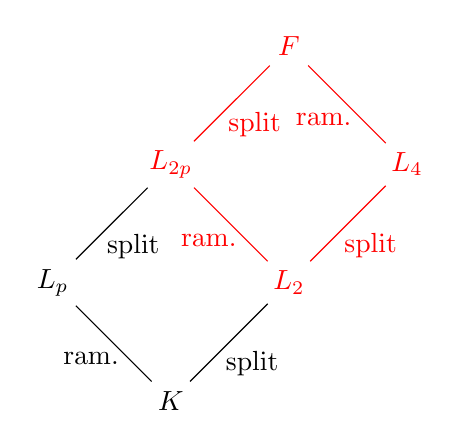
\begin{tikzpicture}

            \node (Q1) at (0,0) {$K$};
            \node (Q2) at (-1.5,1.5) {$L_p$};
            \node [red] (Q3) at (3,3) {$L_4$};
            \node [red] (Q4) at (1.5,1.5) {$L_2$};
            \node [red] (Q5) at (1.5,4.5) {$F$};
            \node [red] (Q6) at (0,3) {$L_{2p}$};
            

            \draw (Q1)--(Q2) node [pos=0.8, below,inner sep=0.4cm] {ram.};
            \draw (Q1)--(Q4) node [pos=0.8, below,inner sep=0.4cm] {split};
            \draw (Q2)--(Q6) node [pos=0.8, below,inner sep=0.4cm] {split};
            \draw [red] (Q3)--(Q5) node [pos=0.8, below,inner sep=0.4cm] {ram.};
            \draw [red] (Q4)--(Q6) node [pos=0.8, below,inner sep=0.4cm] {ram.};
            \draw [red] (Q6)--(Q5) node [pos=0.8, below,inner sep=0.4cm] {split};
            \draw [red] (Q4)--(Q3) node [pos=0.8, below,inner sep=0.4cm] {split};
        \end{tikzpicture}
        \caption[short]{\centering Field diagram for a $C_{4p}$ extension, together with the splitting\\ behaviour of a prime $\pp$ in $L_2$ with $e_\pp=p$ and $f_\pp=1$ over $F$.}
    \end{figure}
\end{proof}

We are now ready to prove Theorem \ref*{thm_consistent_cyclic} for even $d$. We break down the proof into three cases:

\subsubsection*{Case 1: $d$ is not divisible by any odd prime, so $d=2^l$}
If $l=1$, then $\QQ(\zeta_2)=\QQ$, so there is nothing to prove, so assume that $l\geq2$. If $\Gal(F/\QQ)=C_{2^l}$, then 
$$\frac{\prod_i C_{E/F_i}}{\prod_j C_{E/F'_j}}=\frac{C_{E/F}}{C_{E/L_{2^{l-1}}}},$$
and by Lemma \ref*{lem_Cp}, we know that this is a rational square up to factors of $2$, so it suffices to show that $2$ is a norm of every quadratic subfield of $\QQ(\zeta_{2^l})$. A standard argument shows that $\Gal(\QQ(2^l)/\QQ)=(\ZZ/2^l\ZZ)^*=C_{2^{l-2}}\times C_2$ and therefore $\QQ(\zeta_{2^l})$ has $\QQ(i)$ as its unique quadratic subextension if $l=2$ and has three quadratic subextensions if $l\geq 3$. Note that $\zeta_8=(1+i)/\sqrt{2}$ and therefore $\QQ(\zeta_8)=\QQ(i,\sqrt{2})$. The three quadratic subextensions are therefore $\QQ(i), \QQ(\sqrt{2})$ and $\QQ(\sqrt{-2})$. Then the result follows from the fact that 
$$2=\Norm_{\QQ(i)}(1+i)=\Norm_{\QQ(\sqrt{-2})}(2)=\Norm_{\QQ(\sqrt{2})}(2+\sqrt{2}).$$

\subsubsection*{Case 1: $d$ is divisible by at least two odd primes}
Let $K=L_{d/\rad(d)}$ be as in Remark \ref*{rem_radical} such that $\Gal(F/K)=C_{\rad(d)}$ and all fields appearing in the product of local factors contain $K$. Then using the same idea as in Lemma \ref*{lem_Cd_odd}, let 
$$\mathcal{A}=\{L_k\supseteq K:2\nmid [L_k:K]\}\quad\text{and}\quad\mathcal{B}=\{L_k\supseteq K:2\mid [L_k:K]\}.$$
Then the fiels in $\mathcal{A}$ and $\mathcal{B}$ are the intermediate fields of (distinct!) $C_{\rad(d)/2}$ extensions. These are odd cyclic extensions, and therefore by Lemma \ref*{lem_Cd_odd} the contribution is a rational square and therefore the norm of any quadratic extension.

\subsubsection*{Case 3: $d$ is divisible by one odd prime}
In this case, write $d=2^lp^n$ and let $L_k$ be the fields as above. In this case, we note that 
$$\frac{\prod_i C_{E/F_i}}{\prod_j C_{E/F'_j}}=\frac{C_{E/F}C_{E/L_{d/2p}}}{C_{E/L_{d/2}}C_{E/L_{d/p}}}.$$
By Lemma \ref*{lem_Cp}, we know that this product is a square up to multiples of $p$. If $l=1$, then $\Gal(\QQ(\zeta_{2p^n})/\QQ)=(\ZZ/2p^n\ZZ)^*=(\ZZ/p^n\ZZ)^*$ is cyclic, and therefore the unique quadratic subfield is $\QQ(\sqrt{p^*})$, and we already know that $p$ is a norm of this field.

From Lemma \ref*{lem_C2p} that the contribution of $p$ comes from those primes $\pp$ in $L_{d/2p}$ such that they ramify in $L_{d/2}$ and they split in $L_{d/p}$. However, as in the proof of Lemma \ref*{lem_C4p}, the prime $\bar{\pp}=\pp\cap L_{d/4p}$ must also split in $L_{d/2p}$ so $\bar{\pp}=\pp\pp'$ for $\pp'\neq\pp$ in $L_{d/2p}$. Since $\pp$ and $\pp'$ have the same splitting behaviour, they give the same contribution. Hence, the product of local terms is in fact a rational square and therefore the norm of any quadratic extension.

This concludes the proof of Theorem \ref*{thm_consistent_cyclic}, and we have in addition shown that the contribution is always a square except when $d=2^n,p^n$ or $2p^n$, where $p$ is an odd rational prime.
\qed
